%----------------------------------------------------------------------------------------
%	PACKAGES AND OTHER DOCUMENT CONFIGURATIONS
%----------------------------------------------------------------------------------------
\documentclass[a4paper,twoside]{article}

\usepackage{kpfonts}
\usepackage[T1]{fontenc}
\usepackage[utf8]{inputenc}
\usepackage[french]{babel}

\linespread{1.05} % Line spacing
\usepackage{microtype} % Slightly tweak font spacing for aesthetics
\usepackage{paralist} % Used for the compactitem environment which makes bullet points with less space between them

\usepackage[hmarginratio=1:1,top=32mm,columnsep=20pt]{geometry}
\usepackage{multicol}
\usepackage[hang,small,labelfont=bf,up,textfont=it,up]{caption} % Custom captions under/above floats in tables or figures
\usepackage{float} % Required for tables and figures in the multi-column environment - they need to be placed in specific locations with the [H] (e.g. \begin{table}[H])

\usepackage{abstract} % Allows abstract customization
\renewcommand{\abstractnamefont}{\normalfont\bfseries} % Set the "Abstract" text to bold
\renewcommand{\abstracttextfont}{\normalfont\small\itshape\/} % Set the abstract itself to small italic text

\usepackage[colorlinks=true,allcolors=cyan]{hyperref} % For hyperlinks in the PDF
\hypersetup{pdfinfo={Title={Analyse d'une vulnérabilité SSL/TLS: BEAST}, Author={}, Subject={Sécurité des réseaux}, Producer={pdfTeX}}}

\pdfinfoomitdate1
\pdfsuppressptexinfo-1

\usepackage{graphicx}

%----------------------------------------------------------------------------------------
%	TITLE SECTION
%----------------------------------------------------------------------------------------
\title{\vspace{-12.5mm}\fontsize{16pt}{10pt}\selectfont\textbf{Analyse d'une vulnérabilité SSL/TLS: BEAST}\vspace{-1.75em}} % Article title
\author{}
\date{\normalsize 19 septembre 2016}

%----------------------------------------------------------------------------------------

\begin{document}

\maketitle % Insert title

%----------------------------------------------------------------------------------------
%	ARTICLE CONTENTS
%----------------------------------------------------------------------------------------

Le protocole SSL/TLS est aujourd'hui le fondement de la sécurité de nos
échanges sur internet. Il permet l'établissement d'une session sécurisée et
protège les informations sensibles que l'on peut transmettre: mots de
passe, codes de cartes bancaires. Il permet également de protéger notre vie
privée en évitant que nos informations personnelles circulent en clair sur
le réseau.

Il devient si indispensable que l'obtention de certificats qui étaient
jusqu'alors payants ou disponible sous certaines contraintes est maintenant
accessible à tous facilement grâce à des initiatives comme Let's Encrypt,
qui visent à protéger la totalité des sites web et leurs utilisateurs
contre les attaques simples que l'on peut rencontrer sur des réseaux
publics.

Cependant, le protocole TLS a souffert par le passé d'un certain nombre de
failles, qui ont pu permettre à des personnes ou des organisations
malveillantes de déchiffrer des données pourtant protégées par ce
protocole. Dans ce document, nous analyser la vulnérabilité BEAST qui est
l'une d'entre elles.

\section{Contexte}

Nous allons tout d'abord donner quelques informations sur l'historique et
les objectifs du protocole TLS, en s'intéressant notamment au traitement des
messages lors de l'opération de cryptage.

\subsection{SSL/TLS}

SSL (\emph{Secure Sockets Layer}) est un protocole de communication réseau
cryptographique qui utilise une combinaison de clé publique et de
cryptographie symétrique pour assurer une communication sécurisée entre
machines. SSL est utilisé au dessus du protocole TCP/IP qui assure le
transport et le routage de données sur un réseau et en dessous de protocoles
applicatifs comme HTTP ou SMTP dans le cas respectivement de navigation
internet et d'envoi de mails. Il a été initialement introduit par Netscape
dans les années 1990, ce qui a abouti après une refonte à une standardisation par
l'IETF (\emph{Internet Engineering Task Force}) en 1996 sous la révision
SSL 3.0.

Le protocole TLS (\emph{Transport Layer Security}) est une évolution du protocole
SSL pour entrer dans un processus de standardisation plus ouvert et contrer
dans sa première version la vulnérabilité POODLE (\emph{Padding Oracle On
Downgraded Legacy Encryption}) introduite avec SSL 3.0, qui permet à un
attaquant de décrypter des informations sensibles. La dernière révision
disponible actuellement du protocole TLS (ou SSL/TLS) est TLS 1.2 définie en
2008. Protéger une connexion avec TLS a pour objectif de satisfaire les
propriétés suivantes:

\begin{itemize}
    \item la confidentialité des données échangées à l'aide de clés de
	cryptage symétriques, générées pour chaque session à partir d'un
	secret partagé de façon sécurisée au moment du \emph{handshake},
    \item l'authentification des parties mises en jeu (requise au moins
	pour le serveur) à l'aide de clés publiques,
    \item l'intégrité des données échangées pour prévenir leur perte ou leur
	altération durant l'échange en utilisant un code d'authentification
	de message MAC (\emph{Message Authentication Code}).
\end{itemize}

Le protocole TLS est configurable et peut ainsi utiliser différents
algorithmes d'échange de clés, de cryptage des données et de vérification de
l'intégrité des messages qui sont négociés au moment du \emph{handshake}.
Cette partie a été rédigé à l'aide de~\cite{Kaufman:2002:NSP}
et~\cite{Wikipedia:TLS}.

\subsection{CBC}

Les algorithmes de chiffrement peuvent s'appliquer sur des données
arbitrairement longues. Les opérations élémentaires de ces algorithmes, dans
des unités de chiffrage notamment, ne peuvent pas s'appliquer sur la
totalité des données et considèrent ainsi des blocs. La méthode de découpage
des algorithmes de chiffrement par blocs est appelée mode d'opération.

\subsubsection{Généralités}

L'attaque BEAST (\emph{Browser Exploit Against SSL/TLS}) a été démontrée
pour la première fois le 23 septembre 2011 dans le cas de communications en
HTTPS~\cite{Thai:2011:XOR}, bien que son principe fut découvert dès 2002
dans le cas du protocole SSH~\cite{Bellare:2002:AES} et étendue par la
suite au SSL~\cite{Bard:2004:SSL}. Il s'agit d'une attaque à texte clair
connu, c'est-à-dire qu'un attaquant possédant un message chiffré peut
générer à l'aide d'un oracle de cryptage des messages cryptés correspondant
à des messages en clair qu'il a choisi et vérifier s'il y a correspondance.
Cette attaque cible le client dans des échanges comme la navigation web.

L'attaque opère particulièrement sur le mode d'opération par enchaînement
des blocs CBC (\emph{Cipher Block Chaining}), qui est un des modes utilisé
dans les algorithmes de chiffrement par blocs comme AES (\emph{Advanced
Encryption Standard}) ou DES (\emph{Data Encryption Standard}) qui peuvent
être utilisés avec TLS.

\begin{figure}[H]
    \centering
    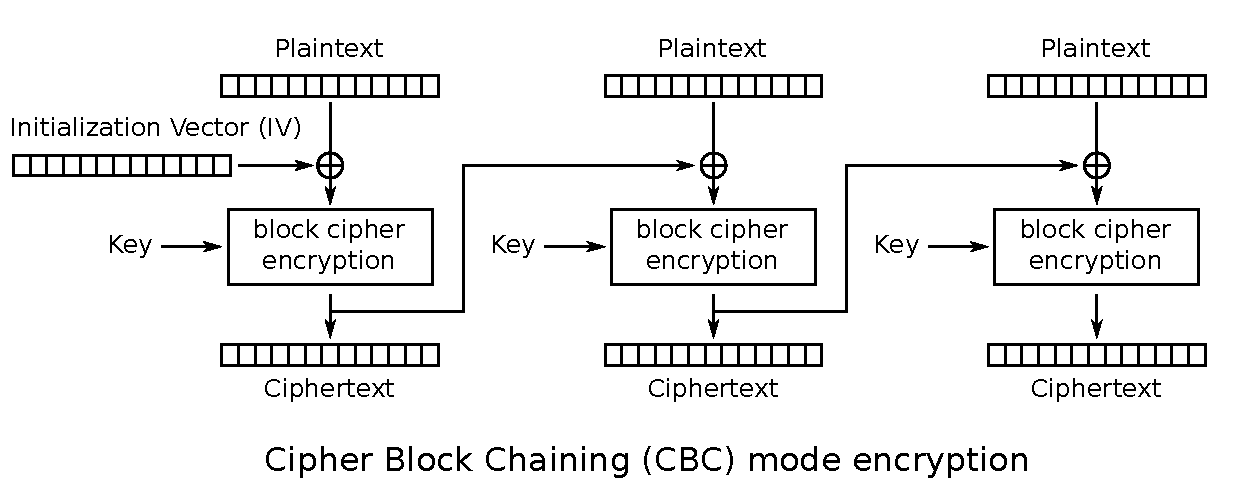
\includegraphics[width=.75\textwidth]{CBC-encryption}
\end{figure}

Pour chiffrer un message, l'algorithme fait appel à un vecteur
d'initialisation (IV) public qui permet d'ajouter de l'aléatoire dans le
cryptage d'un message (la même opération sur un même message donne des
textes chiffrés différents avec des IV distincts). Ce vecteur est utilisé
pour faire un OU-Exclusif $\oplus$ (XOR) avec le bloc de message clair
considéré pour être ensuite crypté avec la clé secrète et sera alors utilisé
de la même façon après le décryptage. La particularité de ce mode par
chaînage est qu'à l'exception du premier bloc de texte considéré, les autres
blocs de textes chiffrés servent de vecteur d'initialisation au bloc
suivant. Un bloc chiffré dépend alors de l'ensemble des blocs chiffrés
obtenus précédemment et du vecteur d'initialisation aléatoire. Les
algorithmes sont conçu pour utiliser un vecteur d'initialisation différent
pour chaque message à chiffrer~\cite{Wikipedia:BCMO}.

\subsubsection{CBC dans TLS}

L'utilisation de CBC dans TLS ne se contente pas de chainer les IV entre les
blocs, mais également entre les messages en prenant le dernier bloc de texte
chiffré du message précédent comme IV du premier bloc du message suivant
(dans l'usage classique du CBC, un nouveau vecteur d'initialisation
aléatoire serait choisi entre les messages à crypter, mais c'est en dehors
du champs de spécification de ce mode et propre à l'implémentation dans
TLS). En considérant un message $P = P_1\ldots P_n$, avec ${(P_i)}_{i\in
\llbracket 1, n \rrbracket}$ de longueur la longueur de bloc de l'algorithme
de chiffrement utilisé. Les blocs de textes chiffrés ${(C_i)}_{i\in
\llbracket 1, n \rrbracket}$ correspondants aux blocs du message en clair
sont calculés avec la fonction de cryptage $E_K$ de la façon suivante:
\begin{equation}
    \label{eq:encryption}
    \left\{\begin{array}{ll}
	C_0 = \text{IV}\\
	C_i = E_K (P_i \oplus C_{i-1})
    \end{array}\right.
\end{equation}

\section{Vulnérabilités}

Nous allons définir formellement le mode d'opération par enchainement de
blocs, esquisser la particularité de TLS dans son utilisation et démontrer
la possibilité d'attaques à texte clair connu et ses conditions de
réalisation avec deux modèles distincts.

\subsection{\emph{Blockwise-Adaptative Chosen-Plaintext}}

Le premier modèle suppose qu'un attaquant peut introduire des blocs à
émettre qu'il a choisi et tenter de deviner le contenu d'une portion du
message en clair~\cite{Bard:2007:BCA}.

\subsubsection{Modèle}

Imaginons que l'on ai accès à un oracle de cryptage et que l'on souhaite
déterminer pour $j\in \llbracket 1, n \rrbracket$ fixé quelconque si le bloc
de texte clair $P_j$ est égal à un certain $P^*$, après avoir observé les
blocs chiffrés ${(C_i)}_{i\in \llbracket 1, n \rrbracket}$. Si l'on chiffre
un nouveau message $P'$ avec $P'_1 = C_{j-1} \oplus C_n \oplus P^*$, alors,
en vertu de l'équation~\ref{eq:encryption}, on obtient le bloc chiffré
suivant:
\begin{align*}
    C'_1    &= E_K (P'_1\oplus C_n)\\
	    &= E_K (C_{j-1} \oplus C_n\oplus P^*\oplus C_n)\\
	    &= E_K (P^*\oplus C_{j-1})
\end{align*}

Or comme $C_j = E_K (P_j\oplus C_{j-1})$, on en déduit que:
\[C'_i = C_j \Leftrightarrow P^* = P_j\]

La conséquence est qu'un attaquant connaissant la forme d'un certain bloc
$P_j$ peut essayer de deviner sa valeur en testant différentes possibilités
et comparer le texte crypté correspondant avec celui du bloc original.

\subsubsection{Conditions d'exploitation}

Une attaquante, Mallory, qui souhaiterait utiliser cette attaque pour
deviner ce qu'Alice envoi à Bob via un protocole utilisant TLS, doit se
soumettre à certaines conditions. D'une part, elle doit identifier le bloc
d'indice $j$ qui contient les données qu'elle souhaite récupérer. Dans le
cas du protocole HTTPS, qui est utilisé sur des sites web sécurisés et
souvent accessibles au public, elle pourrait s'intéresser à simuler de son
côté une session de navigation et regarder le schéma des requêtes qui sont
effectuées pour identifier une portion intéressante.

D'autre part, Mallory doit pouvoir observer le bloc chiffré $C_{j-1}$ pour
pouvoir générer $P'_1$. Heureusement, elle dispose pour cela d'un accès au
réseau par lequel transitent les paquets et utilise une attaque de type
\emph{Man In The Middle}.

Par ailleurs, une fois $P'_1$ généré, elle doit pouvoir insérer ce bloc dans
un message à transmettre. Dans le cas des navigateurs web, ceci pourrait se
faire par un \emph{plugin} malveillant ou tout virus informatique qui pourrait
affecter le comportement du navigateur pour envoyer ce message, en
déclenchant par exemple une requête asynchrone.

À noter que pour que l'attaque fonctionne, ce bloc doit être le premier à
être envoyé puisqu'il doit utiliser le bloc chiffré précédent ($C_{j-1}$).
L'émission de messages depuis l'application n'est pas forcément instantanée
et ils peuvent être ajoutés à une file. Pour cela, il faut tenter d'émettre
quand l'application elle-même fait peu de requêtes (le message est alors
crypté et envoyé immédiatement).

\subsection{\emph{Blockwise Chosen-Boundary Attack}}

Le modèle d'attaque BCBA, qui se base sur la technique du modèle BACP montré
précédemment, suppose maintenant que l'attaquant peut déplacer la frontière
des blocs à l'endroit qu'il souhaite dans le message, ce qui permet de
mettre en place un algorithme déterministe pour décrypter le message
(contrairement à pouvoir seulement deviner une portion ou utiliser la force
brute sur un espace de recherche déterminé mais vaste)~\cite{Thai:2011:XOR}.

\subsubsection{Modèle}

En reprenant le modèle exposé précédemment, on pose $b$ la longueur d'un
bloc. On a donc $|{(P_i)}_{i\in \llbracket 1, n \rrbracket}| = b$. On
considère que l'attaquant peut injecter une donnée $r$ telle que $|r|=b-1$
avant le message $P$. De cette façon, le premier bloc envoyé sera constitué
du message $r$ et du premier octet de $P_1$ : $p_1^1$. On vérifie bien que
$|\langle r, p_1^1\rangle | = b$. Cette étape constitue le déplacement de
frontière.

L'enjeu maintenant est de choisir $P'_1$. Comme il n'y a plus qu'un seul
octet à déterminer dans le bloc, ils suffit de poser $P^{(i+1)}_1 =
C_{j-1}\oplus C_n\oplus P^*_i$, avec $P^*_i = \langle r, i\rangle$. L'indice
$i$ représente les 255 valeurs possibles pour un octet, qu'il suffit alors
de tester indépendamment en réitérant l'opération d'injection.
Au final, avec en moyenne 128 essais nécessaires, on peut déterminer la
valeur de $p_1^1$.

Il est alors aisé d'étendre cet algorithme au déchiffrement de l'ensemble du
message à partir du moment où on ajuste la longueur du préfixe $r$. On peut
alors placer l'octet suivant en dernière position d'un bloc dont il est la
seule inconnue.

\subsubsection{Conditions d'exploitation}

Comme précédemment, Mallory doit disposer de la possibilité d'intercepter
les requêtes chiffrées envoyées par Alice à Bob. Elle doit également pouvoir
déclencher des requêtes et contrôler les frontières des blocs en injectant
ou en contrôlant des données en en-tête du message. Enfin, elle doit pouvoir
ajouter des blocs à des requêtes en cours pour pouvoir utiliser l'attaque à
texte clair connu et déchiffrer le message.

\section{Attaque}

Nous allons détailler l'ataque telle qu'elle a été démontrée pour la
première fois.

\subsection{Le protocole HTTPS}

Le protocole HTTPS peut être vu comme le protocole applicatif HTTP au-dessus
de la couche de cryptage TLS. Les données en texte clair ont donc les mêmes
caractéristiques que le protocole HTTP à savoir:

\begin{itemize}
    \item une ligne correspondant à la requête avec la méthode, le chemin et
	la version HTTP : \texttt{GET /cas HTTP/1.1},
    \item des en-têtes comme \texttt{Cookie: sessionid=1cf1e8dacc3b29c2fc9161baf30539fd;},
    \item une ligne vide,
    \item le corps du message.
\end{itemize}

La donnée généralement fondammentale avec le protocole HTTP est l'en-tête et
en particulier les \emph{cookies}, qui peuvent contenir un identifiant
utilisé par le serveur pour traquer un utilisateur. Le fait de récupérer un
\emph{cookie} qui identifie une session utilisateur peut permettre par
exemple d'accéder à son espace privé qui ne le serait qu'après une étape de
connexion avec identifiant et mot de passe.

\subsection{Scénario}

En tenant compte des conditions d'exploitation présentées à la section
précédente et avec une largeur de bloc de 8 octets, le scénario qui a été
utilisé pour définir le modèle d'attaque est le suivant:

\begin{enumerate}
    \item Alice se rend sur le site de Bob \texttt{https://bob.com/} en
	s'authentifiant, ce qui a pour effet de définir dans son navigateur
	des \emph{cookies} de session.
    \item Alice se rend ensuite sur le site de Mallory
	\texttt{https://mallory.com/} qui contient un logiciel malveillant
	qui permet à cette dernière de décrypter les requêtes HTTPS et
	d'obtenir ses \emph{cookies} en suivant les étapes suivantes:
    \item Mallory déclenche une requête HTTPS de méthode POST du navigateur
	d'Alice vers Bob avec le chemin \texttt{https://bob.com/AAAAAA}, ce
	qui a pour effet d'émettre un message clair $P$ suivant: \texttt{POST
	/AAAAAA HTTP/1.1<CR><LF><REQUEST HEADERS><CR><LF><REQUEST BODY>}. 
    \item Mallory capture le message chiffré $\langle C_1, C_2, \ldots, C_n
	\rangle$ correspondant à $P$, avec notamment $C_3$ le texte
	chiffré
	associé à $P_3 =$ \texttt{P/1.1<CR><LF><X>}. Mallory cherche alors à
	déterminer \texttt{X}, qui est le premier octet de l'en-tête HTTP.
	Pour cela, elle choisit un premier caractère dans l'ensemble des
	caractères autorisés dans les en-têtes.
    \item Mallory possédant le dernier bloc chiffré va générer
	le bloc suivant de texte clair $P^{(i)} = C_{n+i-1}\oplus
	C_2\oplus P^*_i$, avec $P^*_i =$ \texttt{P/1.1<CR><LF><i>}, qu'elle
	va ajouter à la requête en cours. Le navigateur d'Alice va alors
	crypter le bloc et l'envoyer à Bob.
    \item Finalement, Mallory capture le bloc chiffré $C_{n+i-1}$ qu'elle
	compare à $C_3$ pour vérifier sa supposition. S'il n'y a pas
	correspondance, Mallory va retourner à l'étape précédente en
	utilisant une nouvelle valeur possible $i$ pour l'octet inconnu
	\texttt{X}.
\end{enumerate}

On constate que Mallory peut à l'étape 3 contrôler un préfixe pour aligner
la frontière du bloc en utilisant le chemin HTTP de la requête (quitte à
ajouter des paramètres GET inutiles si le serveur bloque la requête dans le
cas où le chemin est invalide).

L'enjeu est alors de savoir s'il existe un adversaire réel qui possède les
mêmes privilèges que Mallory. En particulier, il s'agit de savoir s'il est
possible de développer le logiciel malveillant présent sur le site de
Mallory.

\subsection{Données collectées}

Le scénario présenté s'attaque aux \emph{cookies} de navigation présents
dans l'en-tête HTTP, mais il pourrait s'appliquer de la même façon pour la
suite du message en supposant un temps d'attaque suffisant. Il est
généralement considéré que les \emph{cookies} constituent les données les
plus sensibles puisqu'ils peuvent permettre de réutiliser une session de
navigation et donc à posteriori d'accéder directement au contenu.

Une autre donnée qui aurait pu être la cible d'un telle attaque sont les
mots de passes en clair (dans le message crypté) qui sont envoyés au
serveur lors de la connexion, mais cela nécessiterait un scénario plus
élaboré pour déchiffrer les requêtes dès la connexion au site.

Enfin cette attaque n'est pas spécifique au protocole HTTPS, mais bien à
l'ensemble des protocoles qui utilisent TLS (vulnérables au chaînage d'IV
entre message avec CBC). Dans l'élaboration d'une preuve de concept, cette
attaque a été implémenté à l'aide d'une version préliminaire de l'API
WebSockets d'HTML 5 en utilisant le chaînage des IV (il n'est pas
nécessaire de contrôler tous les bits du premier bloc et il est possible
d'utiliser le second bloc pour tester les hypothèses).

\subsection{Mise en pratique}

Les navigateurs imposent des mesures de sécurité pour contrer les attaques
CSRF (\emph{Cross-Site Request Forgery}), qui empêchent un utilisateur de soumettre
une requête vers un site à partir d'une source d'origine (un autre site internet) non
autorisée par le serveur de destination. L'implémentation historique
avait pour but d'empêcher purement et simplement l'interaction de deux pages
web différentes selon la \emph{Same-Origin Policy}, définie comme la
combinaison protocole, hôte et port.

Notre scénario exige cependant qu'une requête soit émise depuis le site de
Mallory vers celui de Bob, ce qui implique de contourner cette sécurité. La
manière avec laquelle cela a été réalisé lors de la démonstration effectuée
à la Black Hat est d'utiliser une faille \emph{0-day} dans la JVM
(\emph{Java Virtual Machine}), c'est-à-dire une faille exploitée avant que
le créateur du logiciel soit au courant de son existence. Cette faille
permet justement de contourner la SOP dans un \emph{applet} Java qui
s'exécute sous forme de \emph{plugin} dans le navigateur et donc de mener à
bien cette attaque (la démonstration a utilisé le site Paypal en ciblant un
utilisateur)~\cite{Thai:BEAST}.

\section{Correction de la vulnérabilité}

Un certain nombre de freins ont été rencontrés pour migrer vers des protocoles et
des logiciels supportant une version corrigeant cette vulnérabilité.

\subsection{Recommandations}

Deux mesures sont suffisantes pour remédier à cette attaque:

\begin{enumerate}
    \item utiliser correctement CBC en générant à chaque fois un nouvel IV
	pour chaque message. Un candidat pourrait être un \emph{hash} de la
	clé privé et du dernier bloc crypté généré.
    \item utiliser un mode d'opération différent de CBC.
\end{enumerate}

\subsection{TLS 1.1}

La solution privilégiée pour TLS 1.1 est d'utiliser des IV explicites.
Chaque message possède un block chiffré supplémentaire initial qui
correspond à son IV. Ceci correspond à la recommandation 1.

Malheureusement, l'adoption de TLS 1.1 et TLS 1.2 a été laborieuse,
principalement par le temps de réactivité trop long pour leur
implémentation dans les navigateurs (étant donné que la vulnérabilité cible
la partie client), mais également à cause de problèmes de compatibilité
avec des versions d'Internet Explorer, alors que le protocole et son
implémentation dans OpenSSL étaient prêtes.

\subsection{Atténuation}

Des mesures d'atténuation ont donc été mises en place pour pouvoir continuer
à utiliser TLS 1.0. La première recommandation qui a été effectuée est
d'utiliser de préférence l'algorithme de chiffrement à flot RC4
(\emph{Rivest Cipher 4}), qui s'est malheureusement avéré être vulnérable à
un certain nombre d'attaques.

La deuxième pratique qui avait été implémentée dans OpenSSL avant même la
première exploitation de la vulnérabilité est d'utiliser un bloc vide en
début de message, qui n'est pas utilisé en tant que donnée mais est
équivalent à la génération d'un nouvel IV. Pour les mêmes raisons
d'incompatibilité avec Internet Explorer, cette mesure n'était pas activée
par défaut.

La dernière solution qui conserve une compatibilité totale avec TLS 1.0 est
la technique du \emph{1/n-1 split}, qui consiste à envoyer seulement le
premier octet du message dans le premier bloc, et le reste dans le suivant,
qui selon la définition de la structure d'un bloc chiffré utilisera le
premier octet chiffré suivi du MAC comme IV, ce qui le rend suffisamment
aléatoire~\cite{Mozilla:BEAST}.

\section{Conclusion}

Il ressort de cette étude qu'il est difficile d'évaluer ou de prévoir la
faisabilité d'une attaque informatique exploitant une vulnérabilité. Avec
son principe de fonctionnement décrit presque 10 ans à l'avance,
l'exploitation de BEAST a mis non seulement en évidence que le protocole TLS
peut être en pratique vulnérable, mais a surtout montré que la réponse de la
communauté et des industriels peut être particulièrement lente, face à des
solutions \emph{open source} qui avaient déjà pris les devant.

Par ailleurs on peut s'interroger sur la complexité relative entre cette
attaque, dont la mise en œuvre efficace a tout de même nécessité une faille
\emph{0-day} contournant le mécanisme de SOP, par rapport à d'autre attaques
physiques ciblant le matériel ou des chevaux de Troie moins élaborés. Une
extension de ce travail consisterait à analyser des failles dans TLS
découvertes ultérieurement et leur impact, ainsi que certaines améliorations
dans les garanties des algorithmes de chiffrement utilisé avec notamment la
\emph{forward secrecy}, pour assurer que des communications ne puissent pas
être décrypté ultérieurement même si la clé utilisée venait à être
compromise.

%----------------------------------------------------------------------------------------
%	REFERENCE LIST
%----------------------------------------------------------------------------------------
\newpage
\small
\nocite{*}
\bibliographystyle{alpha}
\bibliography{main}
%----------------------------------------------------------------------------------------
\end{document}
